\chapter{Sparsity Patterns of Matrix Sets}
\label{app:sparsity-patterns}

\newpage


\begin{figure}[htpb]
\centering
	\begin{tabular}{cc}
		\subfloat[pwr-3d]{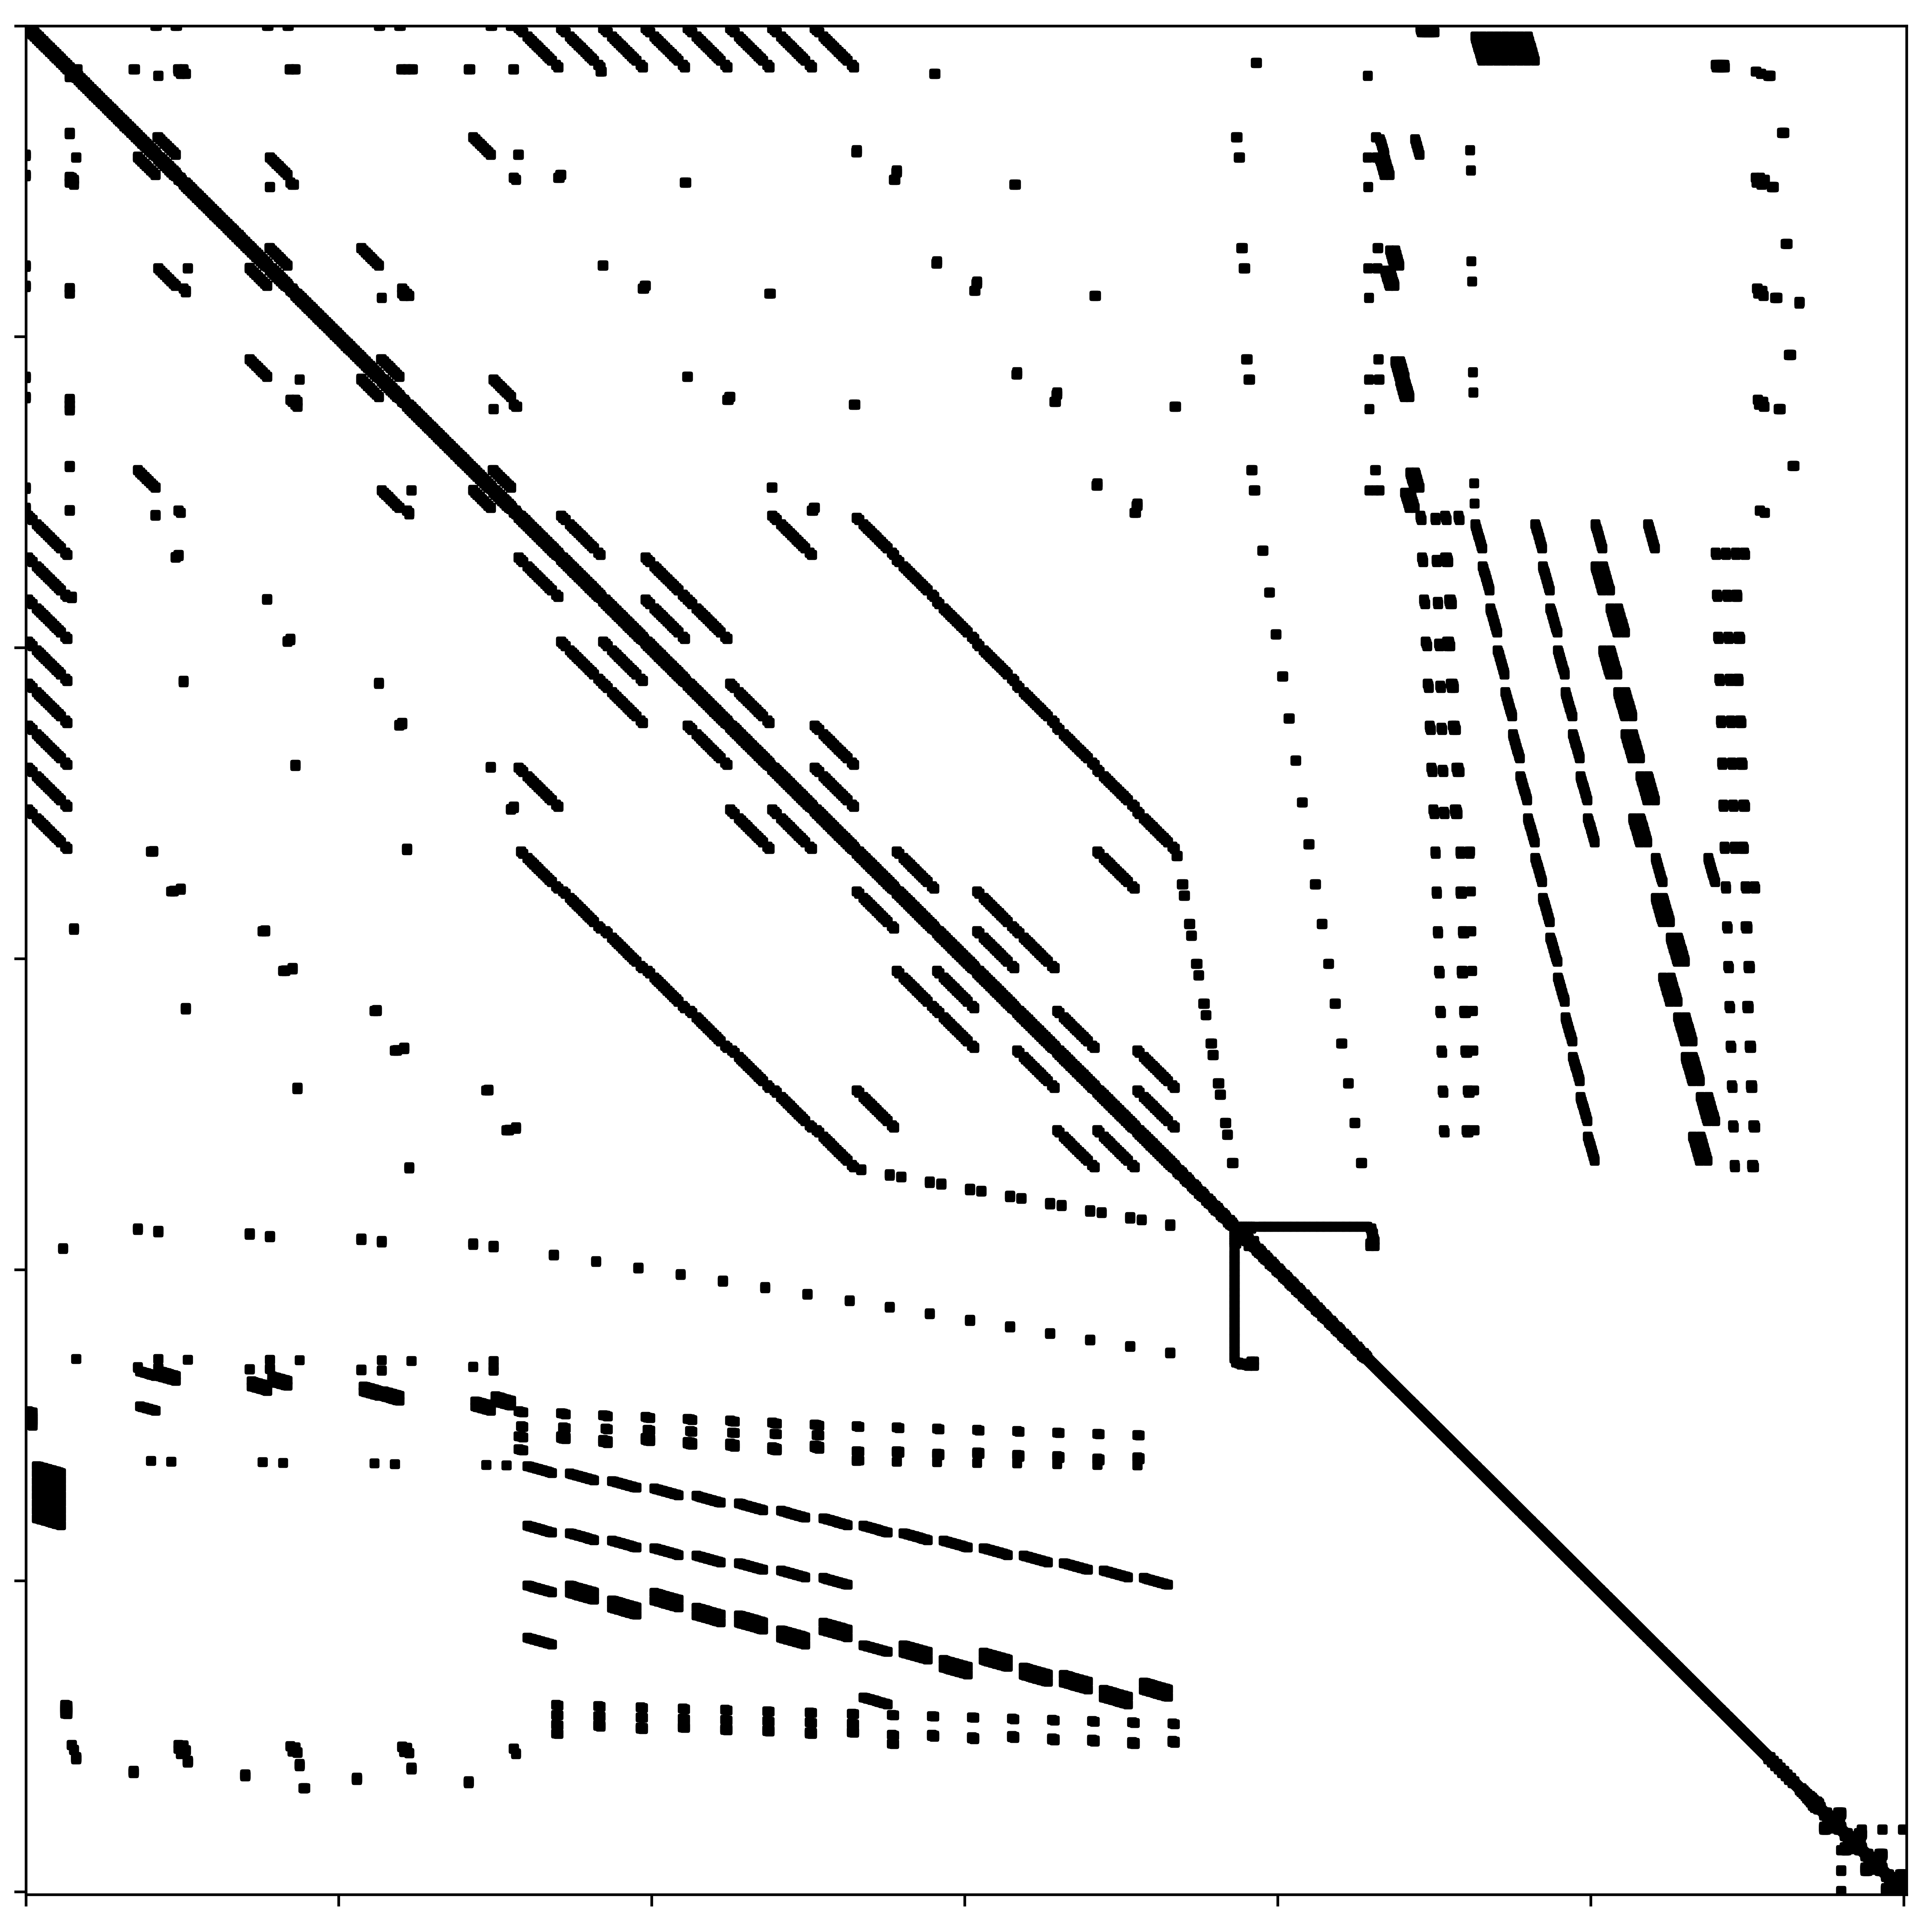
\includegraphics[width=0.32\textwidth]{figures/sparsity-patterns/pwr-3d.png}} &
		\subfloat[cube-5]{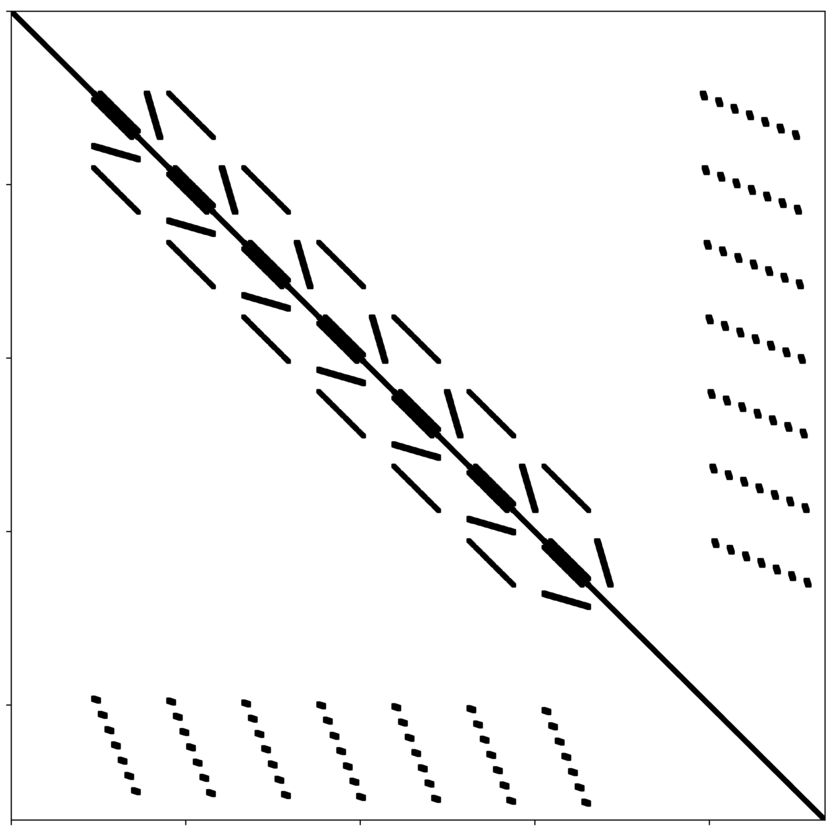
\includegraphics[width=0.32\textwidth]{figures/sparsity-patterns/cube-5.png}} \\
		\subfloat[k3-2]{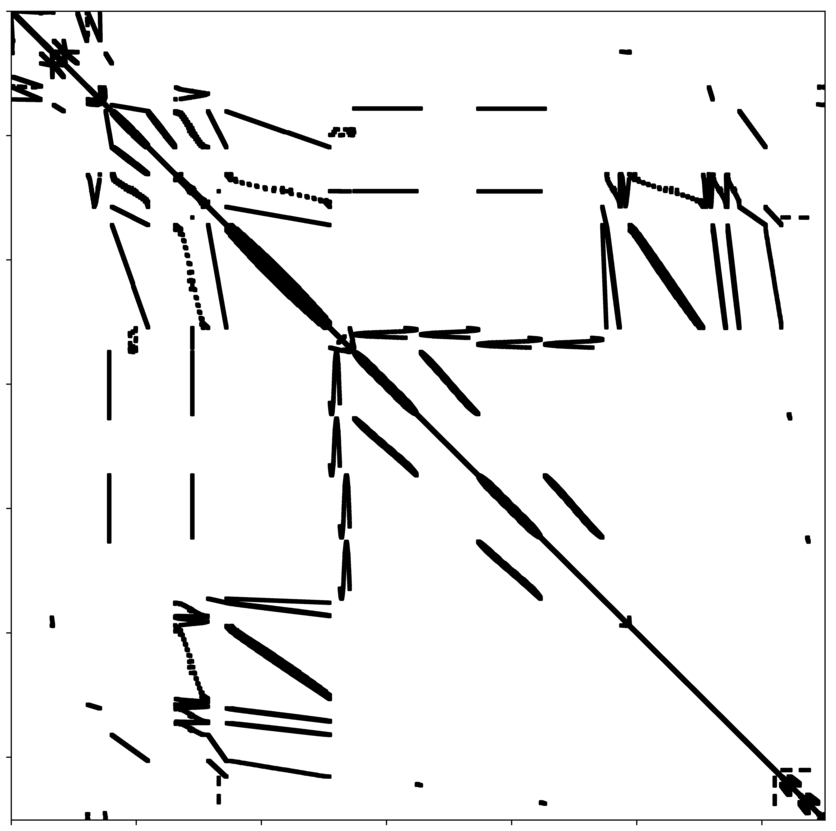
\includegraphics[width=0.32\textwidth]{figures/sparsity-patterns/k3-2.png}} &
		\subfloat[cube-64]{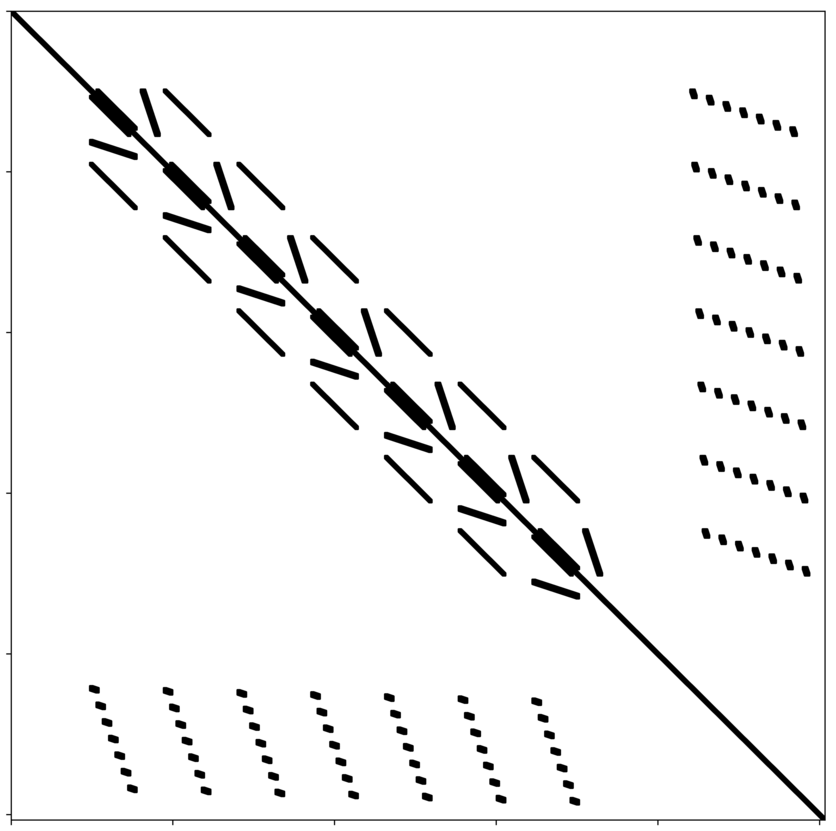
\includegraphics[width=0.32\textwidth]{figures/sparsity-patterns/cube-64.png}}  \\
		\subfloat[k3-18]{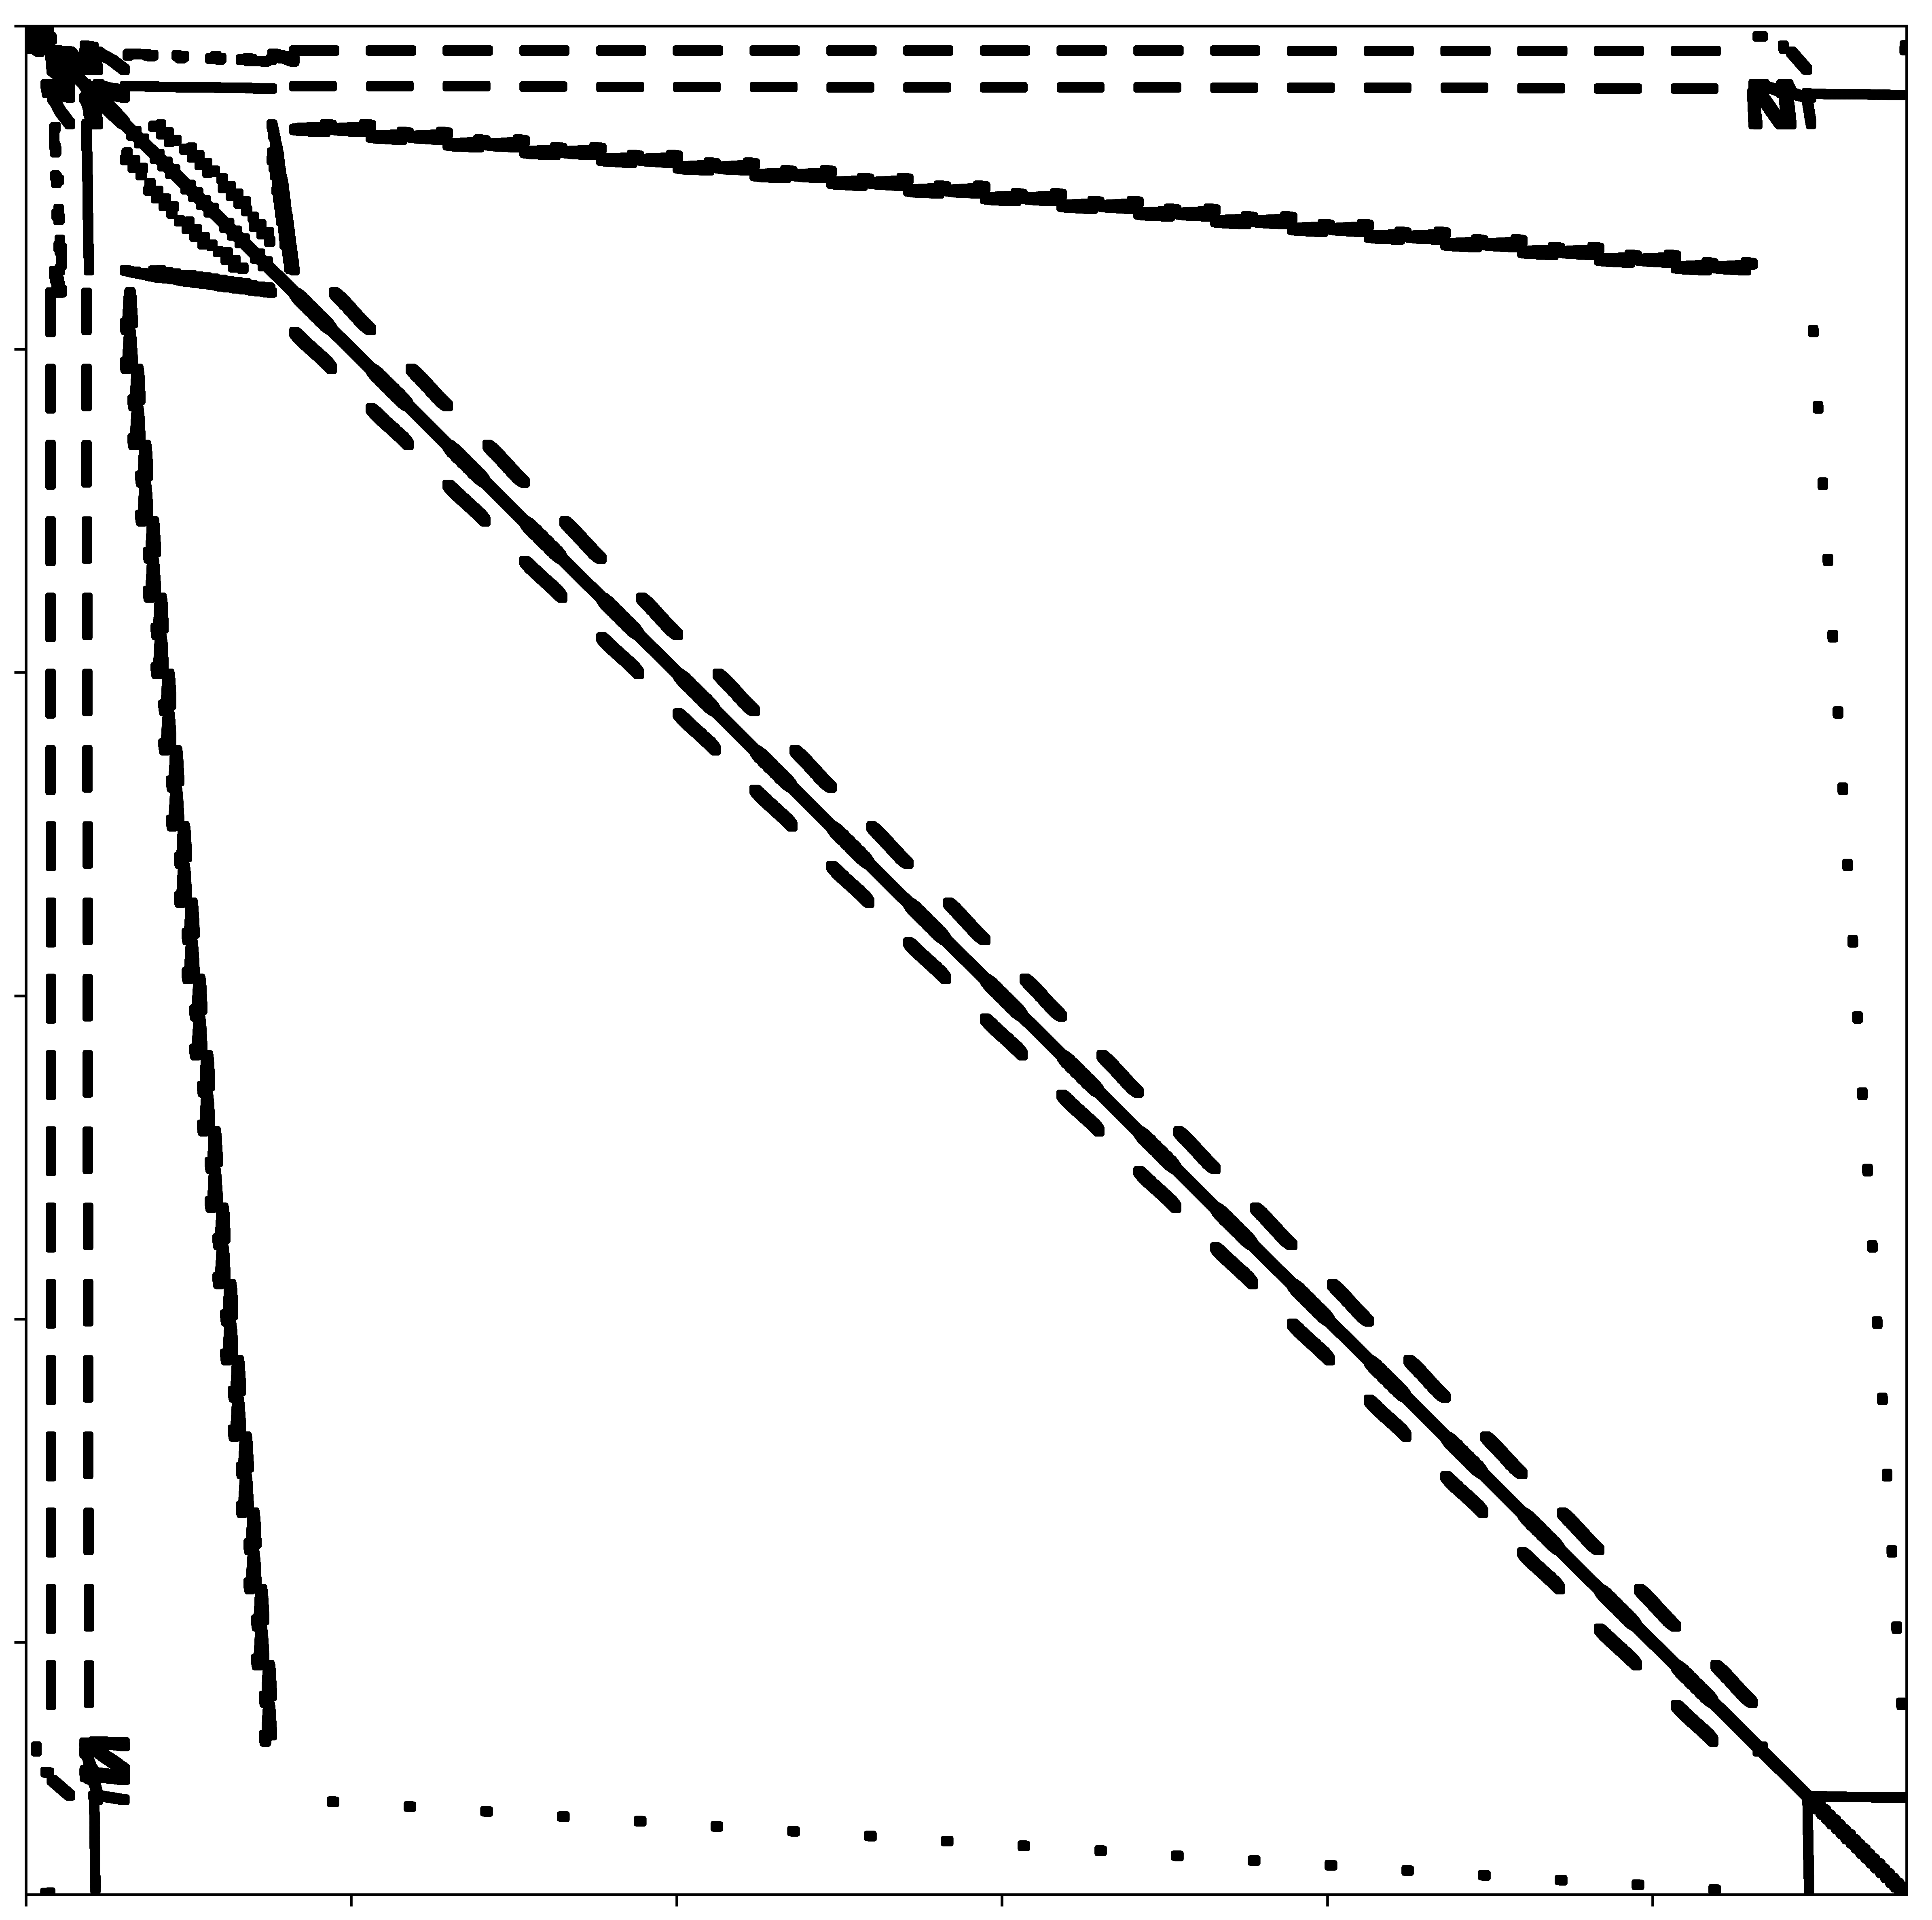
\includegraphics[width=0.32\textwidth]{figures/sparsity-patterns/k3-18.png}} &
		\subfloat[cube-645]{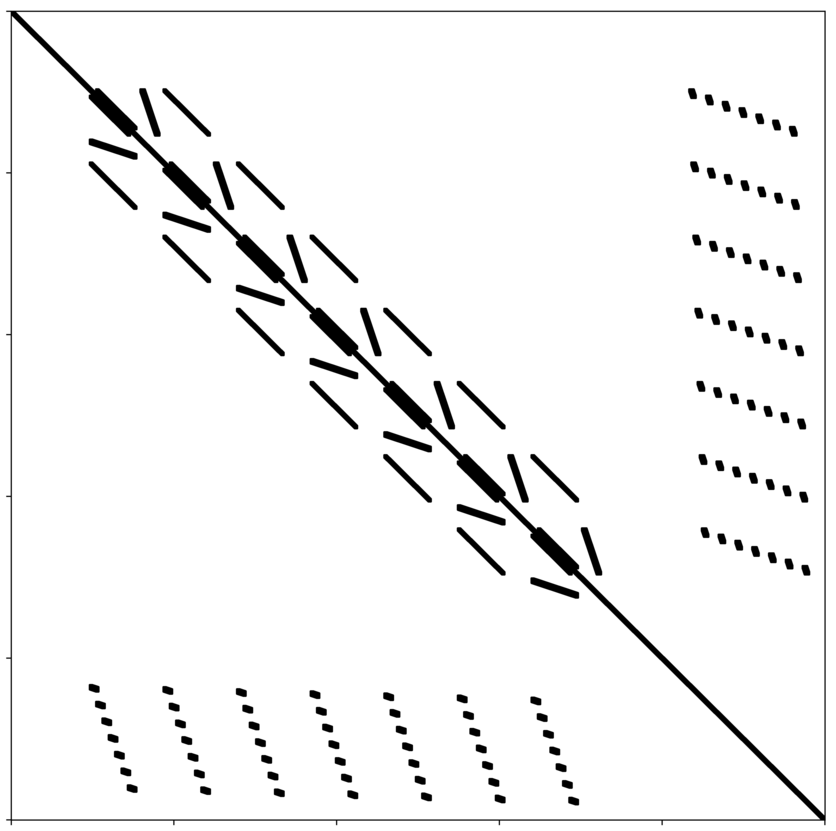
\includegraphics[width=0.32\textwidth]{figures/sparsity-patterns/cube-645.png}} \\
	\end{tabular}
	\caption{Sparsity patterns of GRS matrix set}
	\label{fig:sparsity-pattern-grs}
\end{figure}



\begin{figure}[htpb]
\centering
	\begin{tabular}{ccc}
		\subfloat[cant]{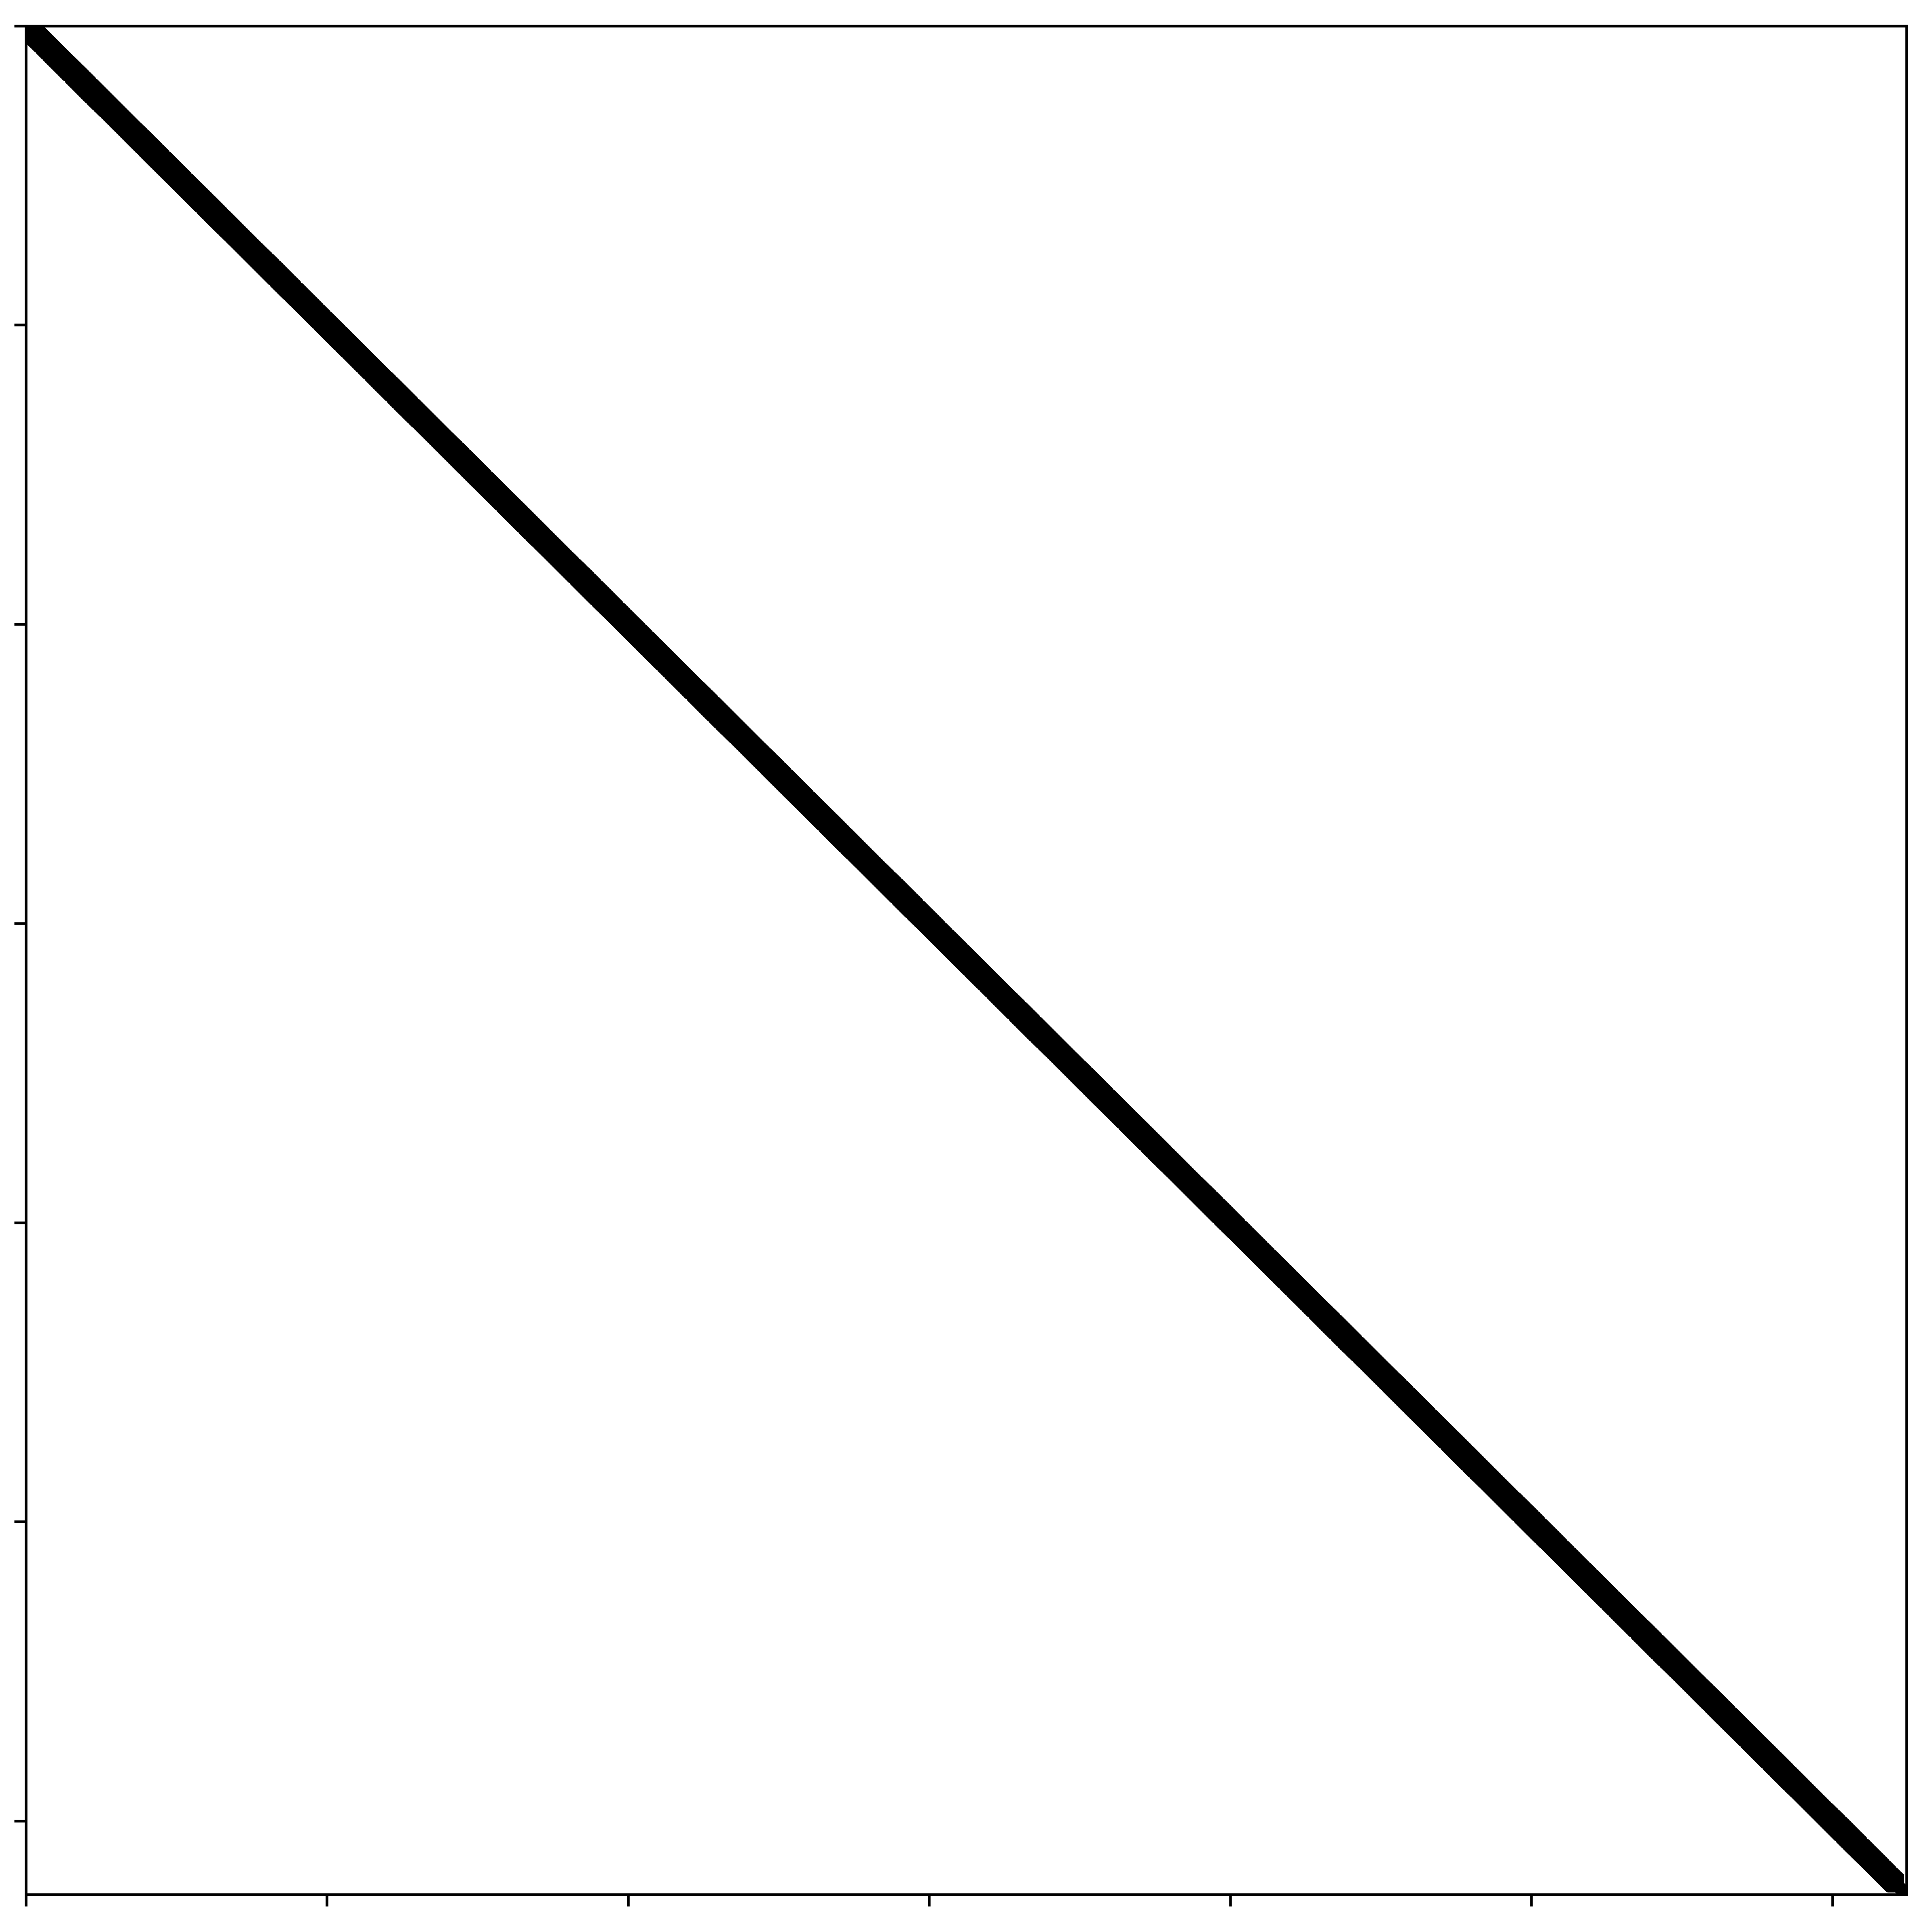
\includegraphics[width=0.32\textwidth]{figures/sparsity-patterns/cant.png}} &
		\subfloat[consph]{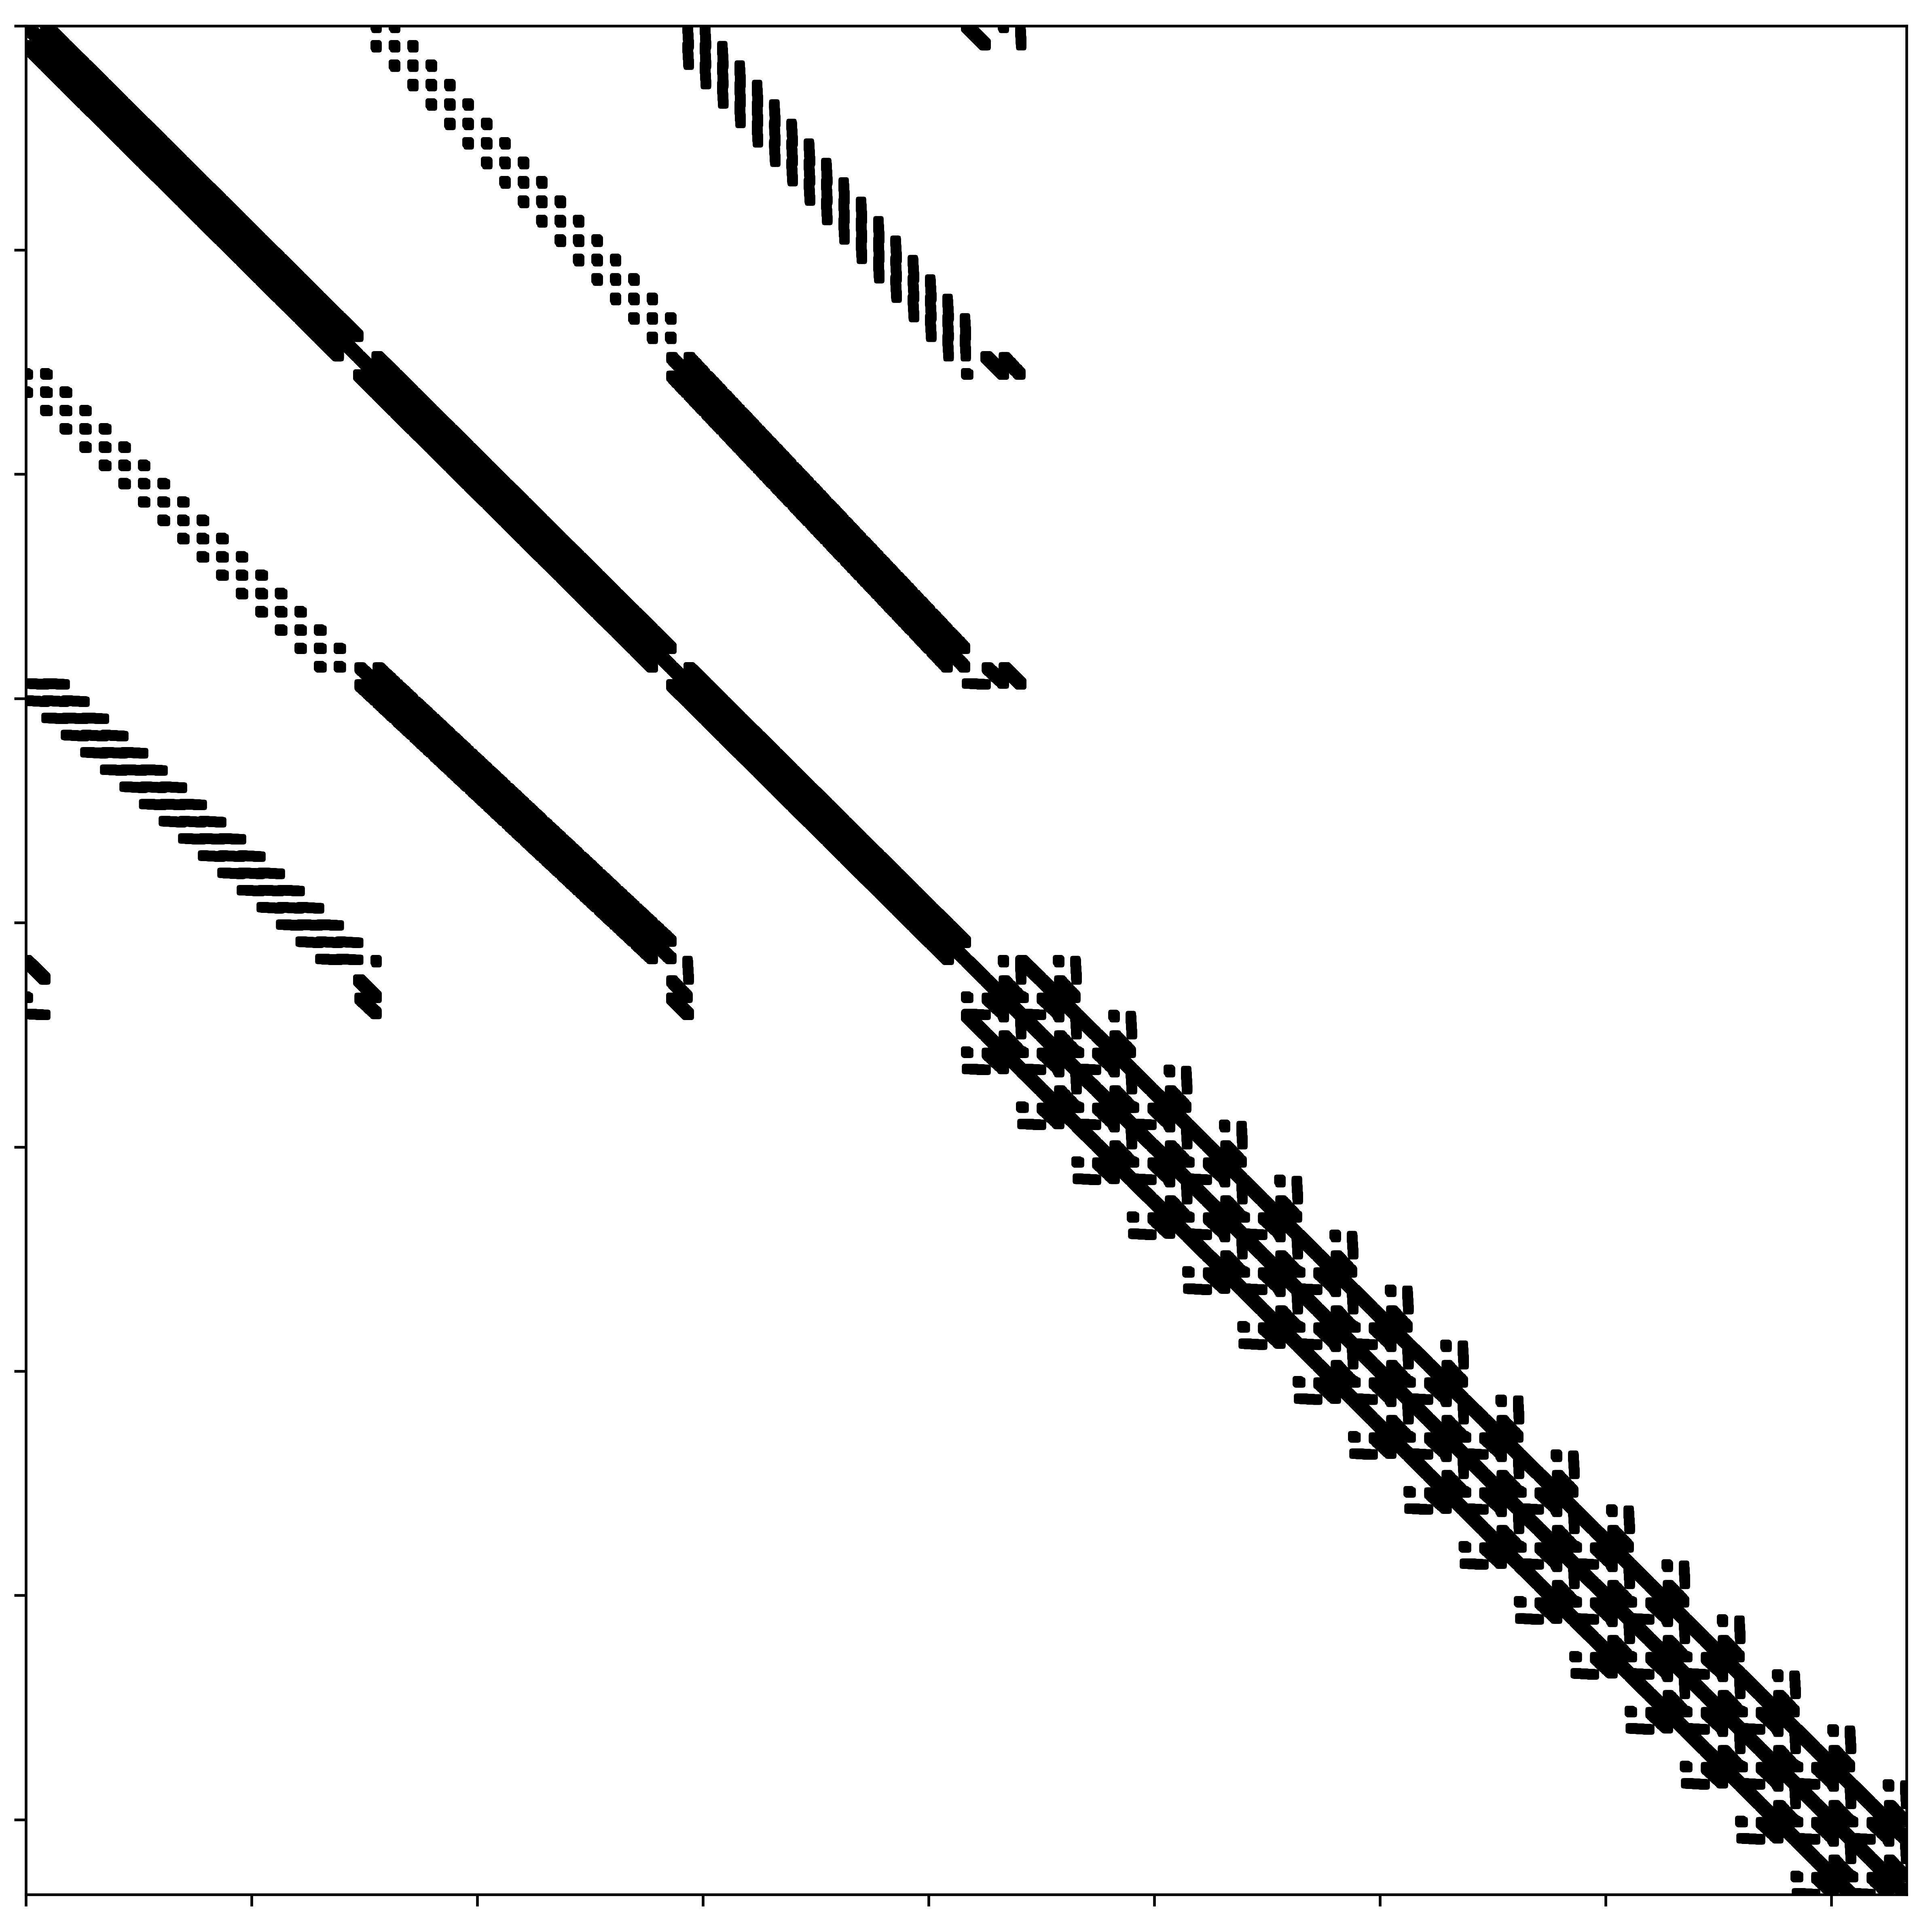
\includegraphics[width=0.32\textwidth]{figures/sparsity-patterns/consph.png}} &
		\subfloat[CurlCurl\_3]{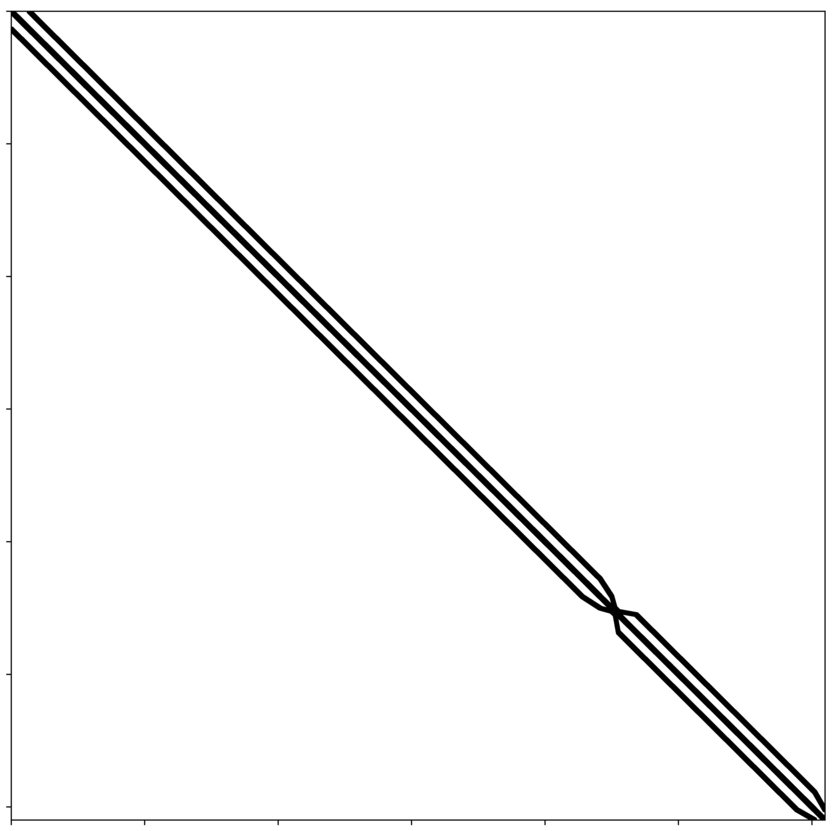
\includegraphics[width=0.32\textwidth]{figures/sparsity-patterns/CurlCurl_3.png}} \\
		\subfloat[Geo\_1438]{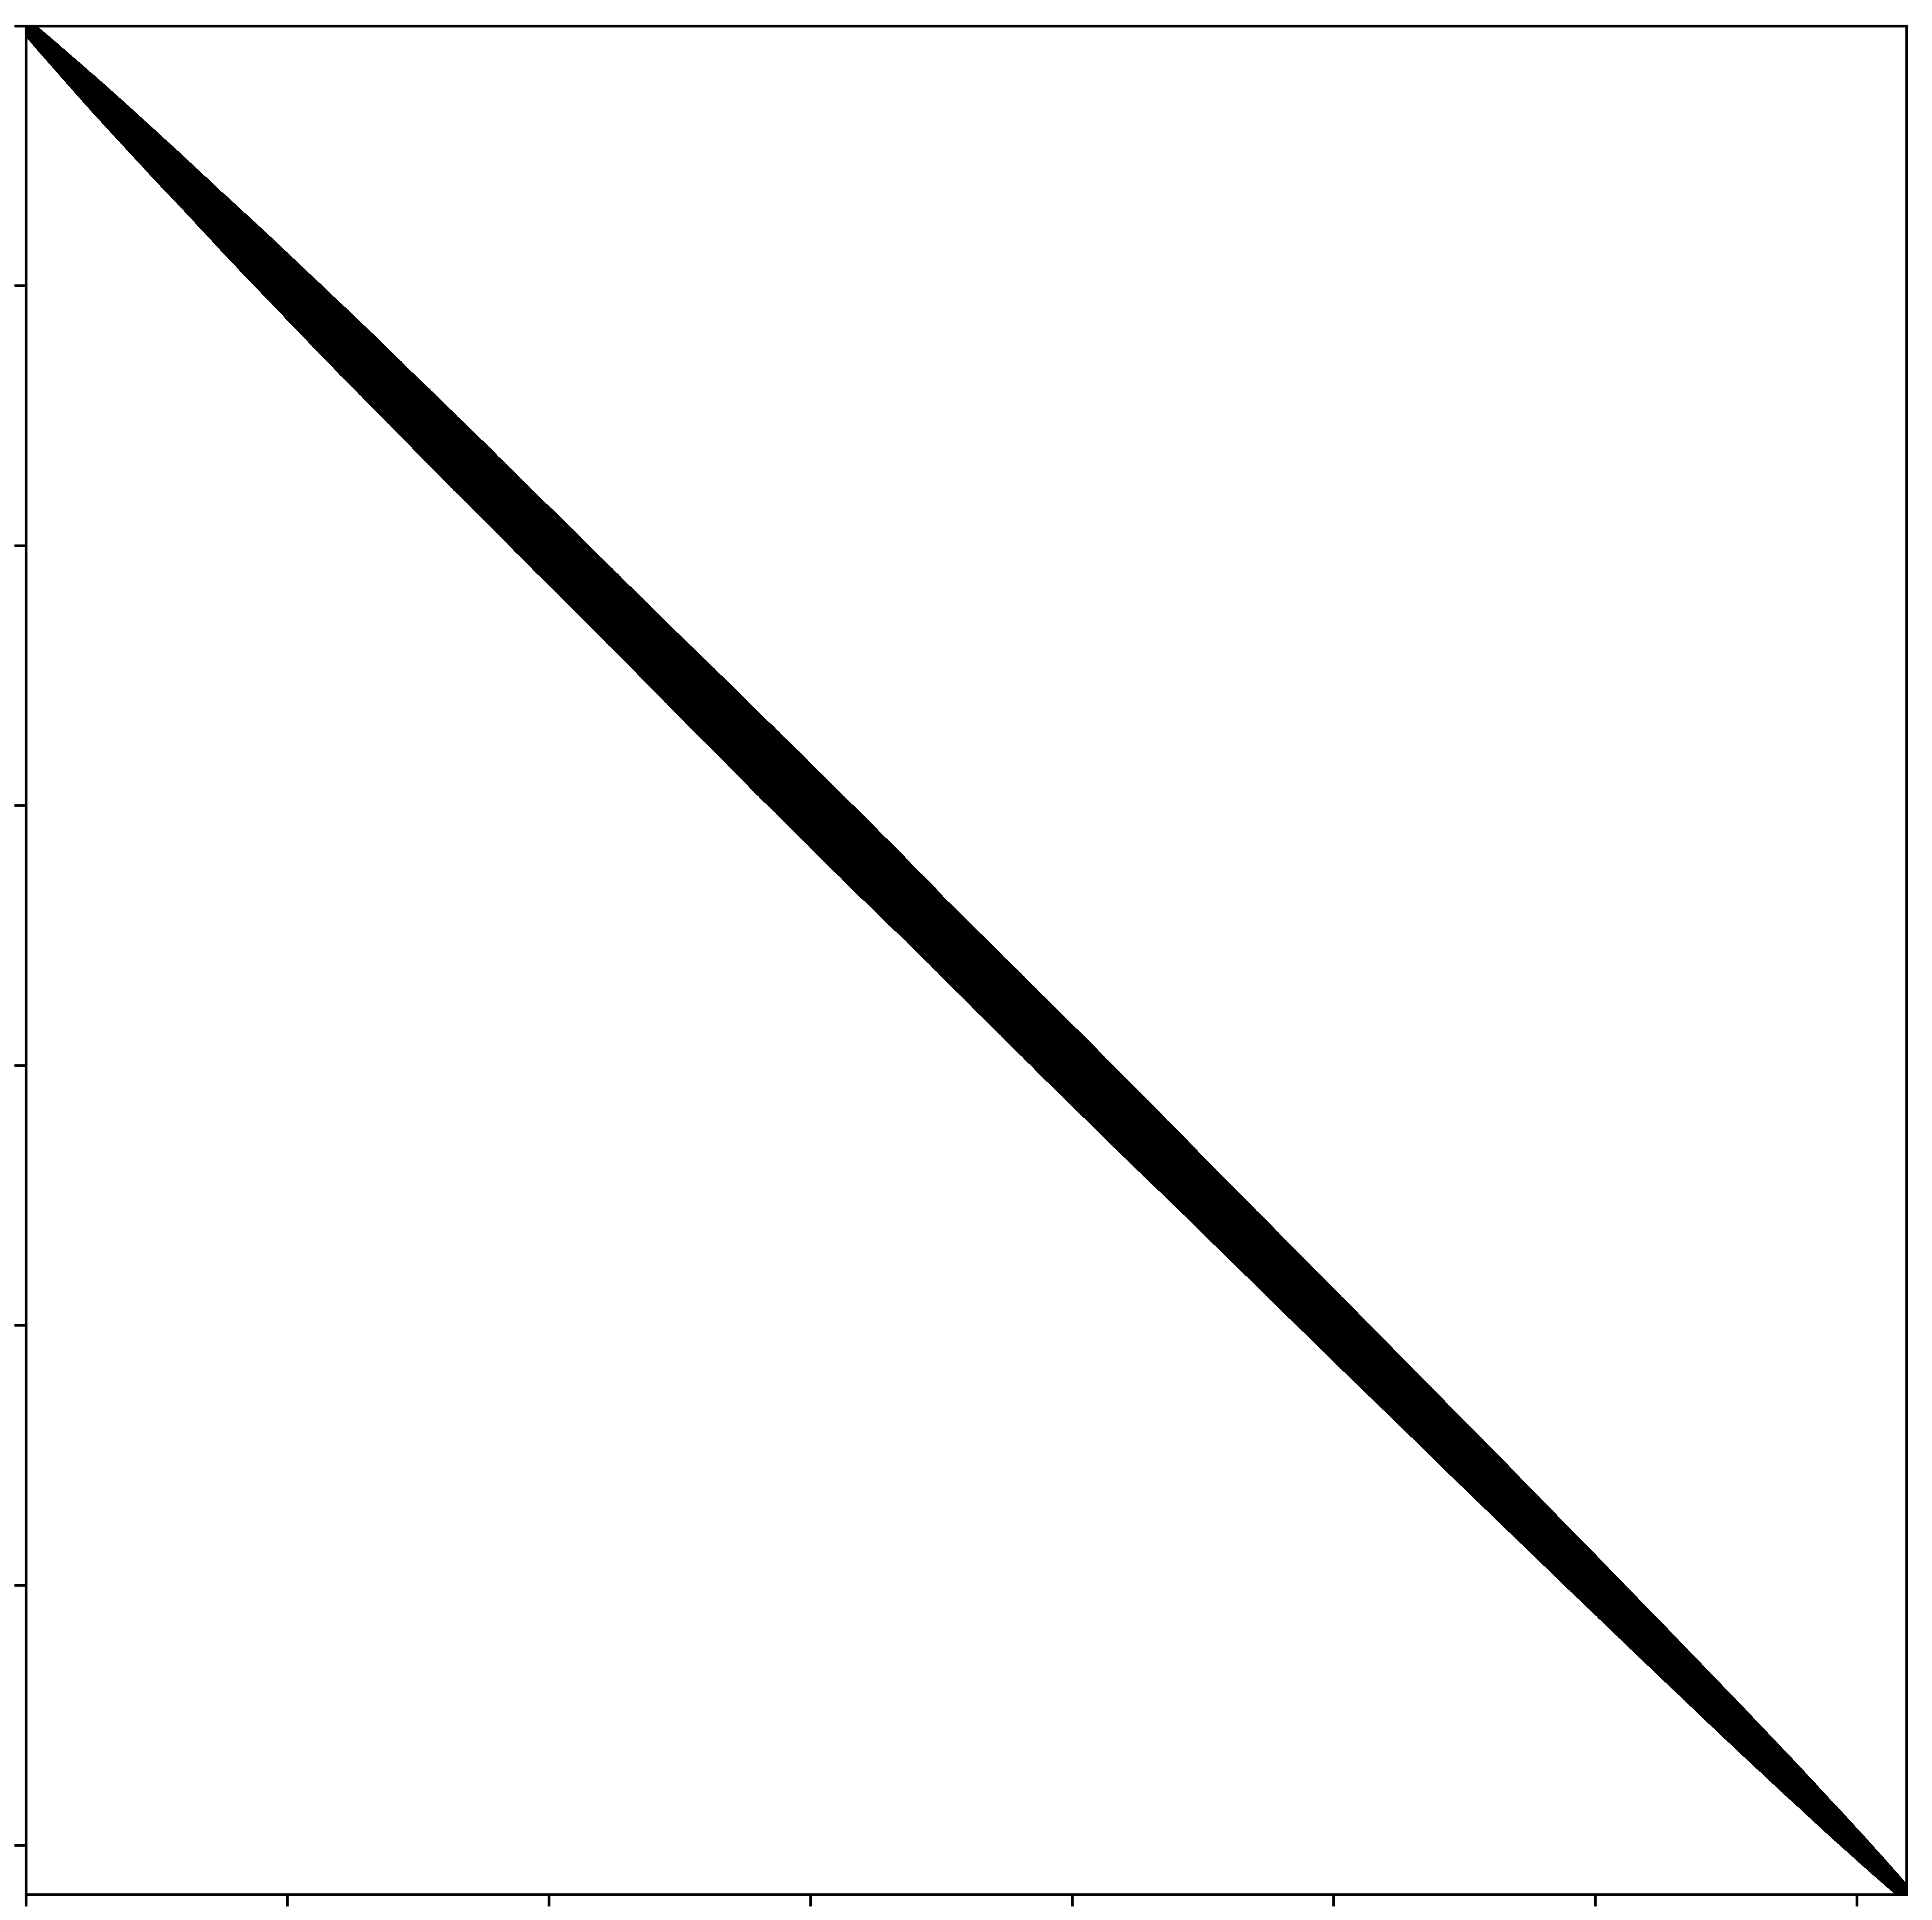
\includegraphics[width=0.32\textwidth]{figures/sparsity-patterns/Geo_1438.png}} &
		\subfloat[memchip]{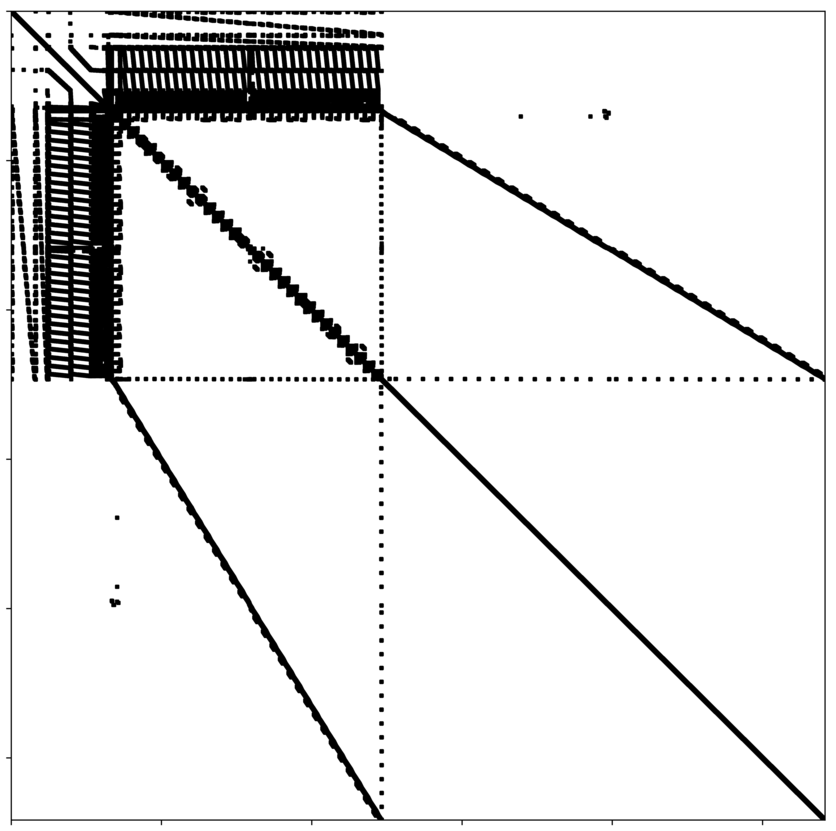
\includegraphics[width=0.32\textwidth]{figures/sparsity-patterns/memchip.png}} &
		\subfloat[PFlow\_742]{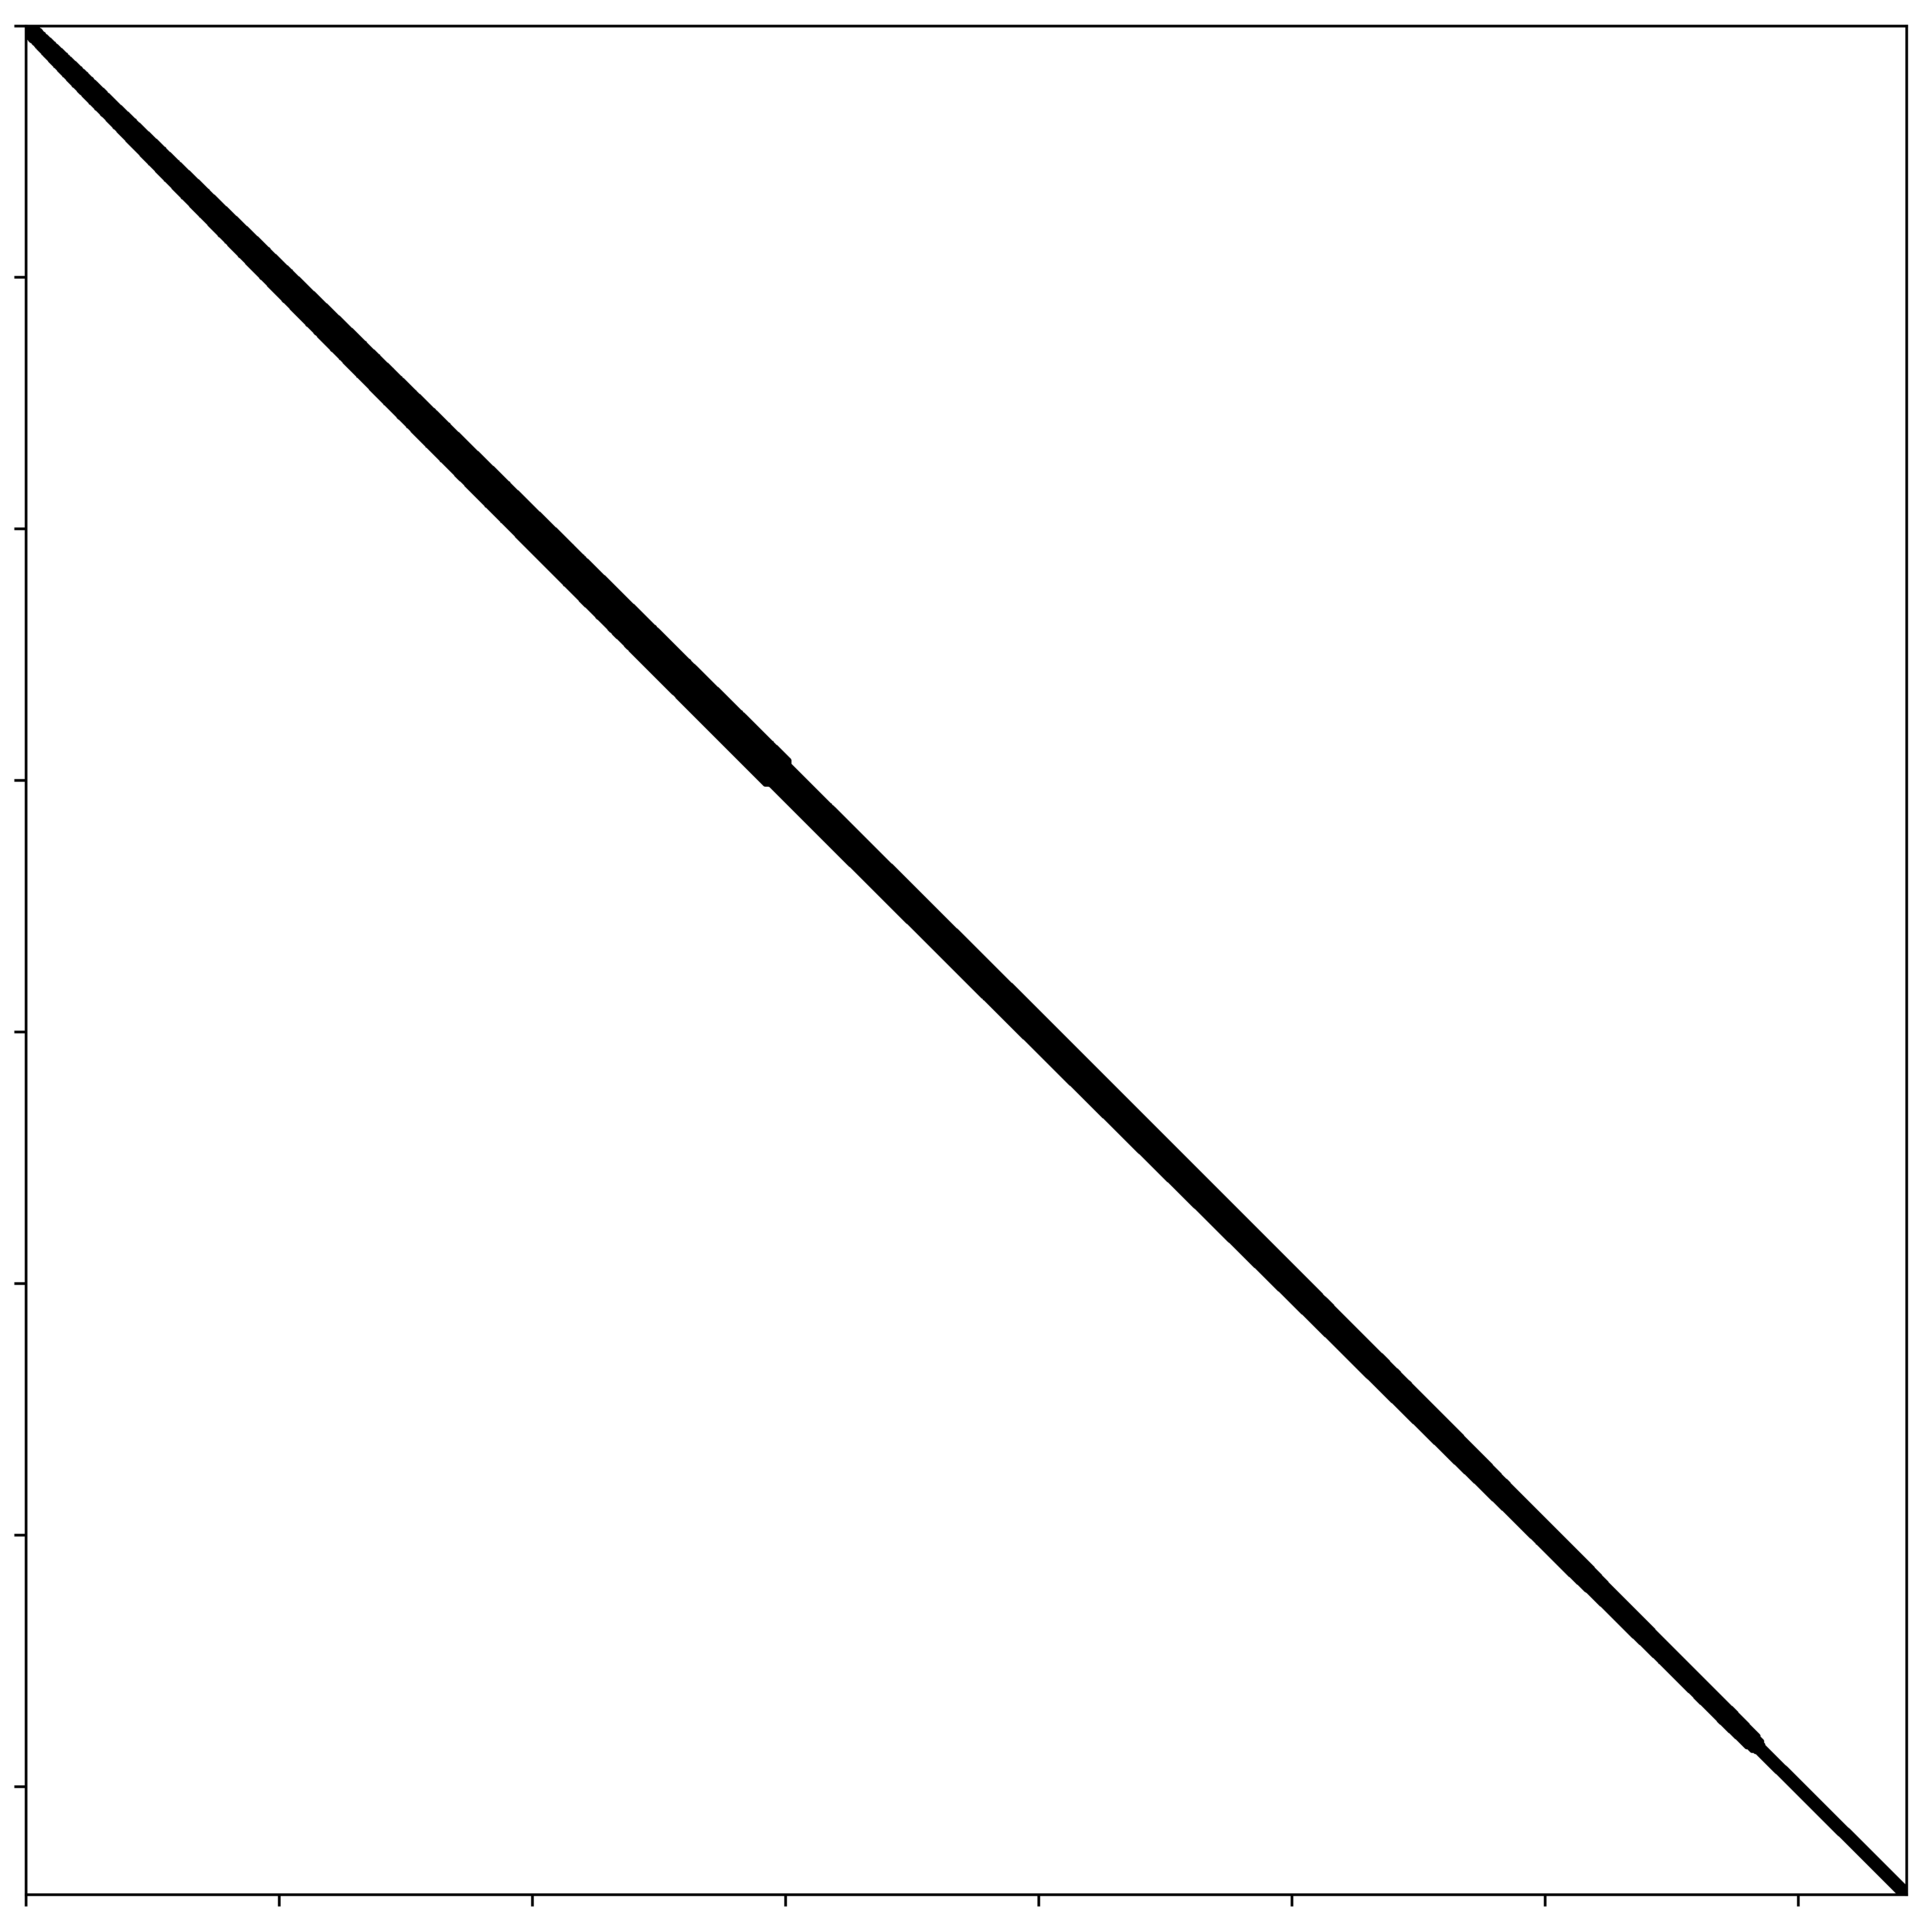
\includegraphics[width=0.32\textwidth]{figures/sparsity-patterns/PFlow_742.png}} \\
		\subfloat[pkustk10]{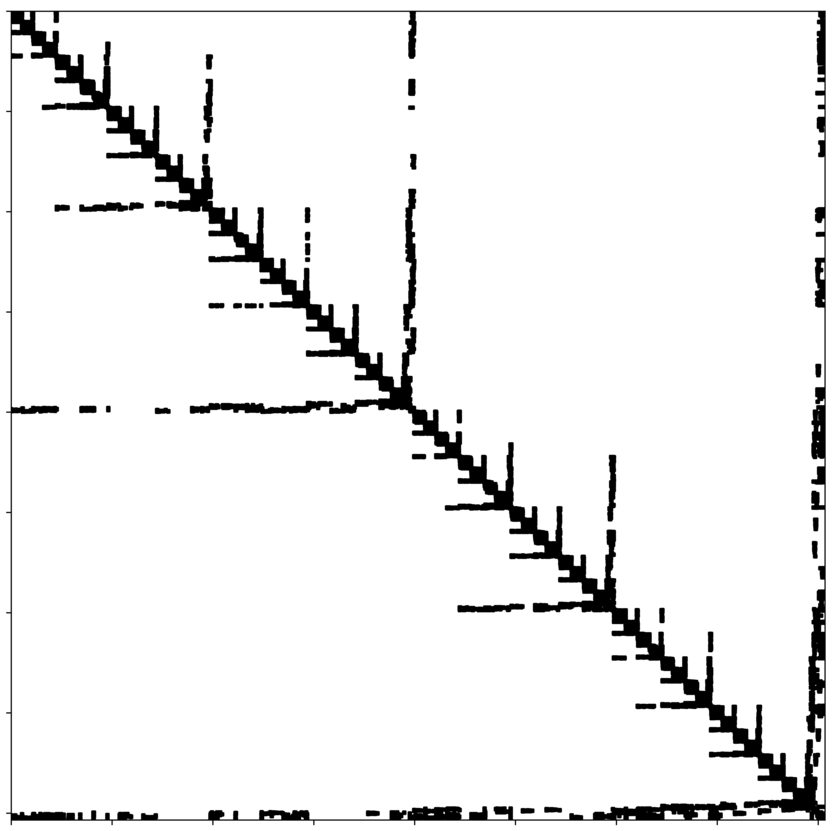
\includegraphics[width=0.32\textwidth]{figures/sparsity-patterns/pkustk10.png}} &
		\subfloat[torso3]{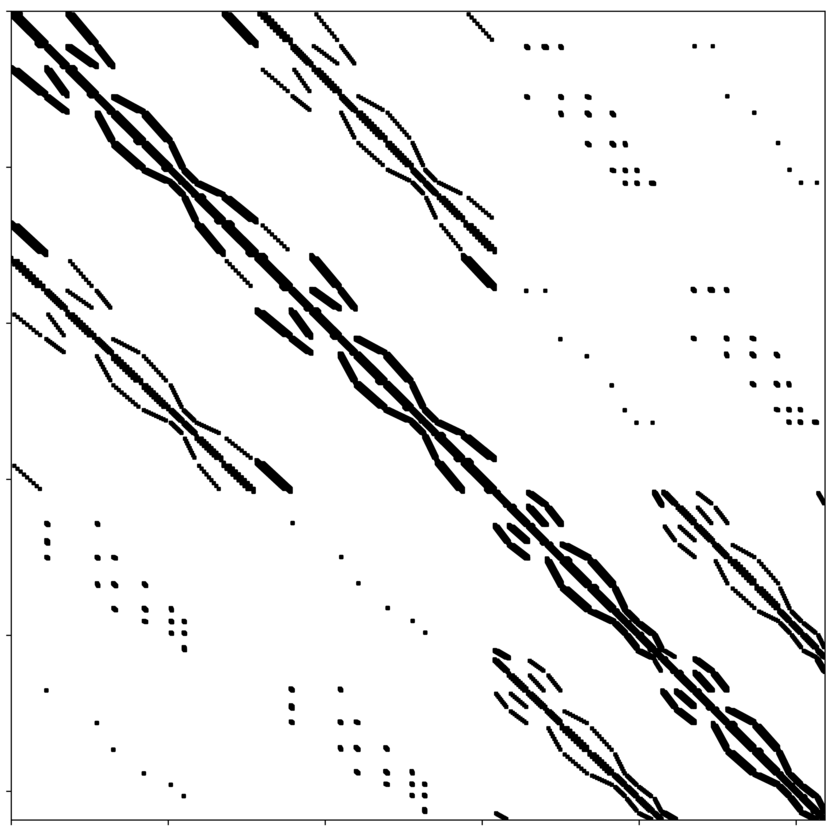
\includegraphics[width=0.32\textwidth]{figures/sparsity-patterns/torso3.png}} &
		\subfloat[x104]{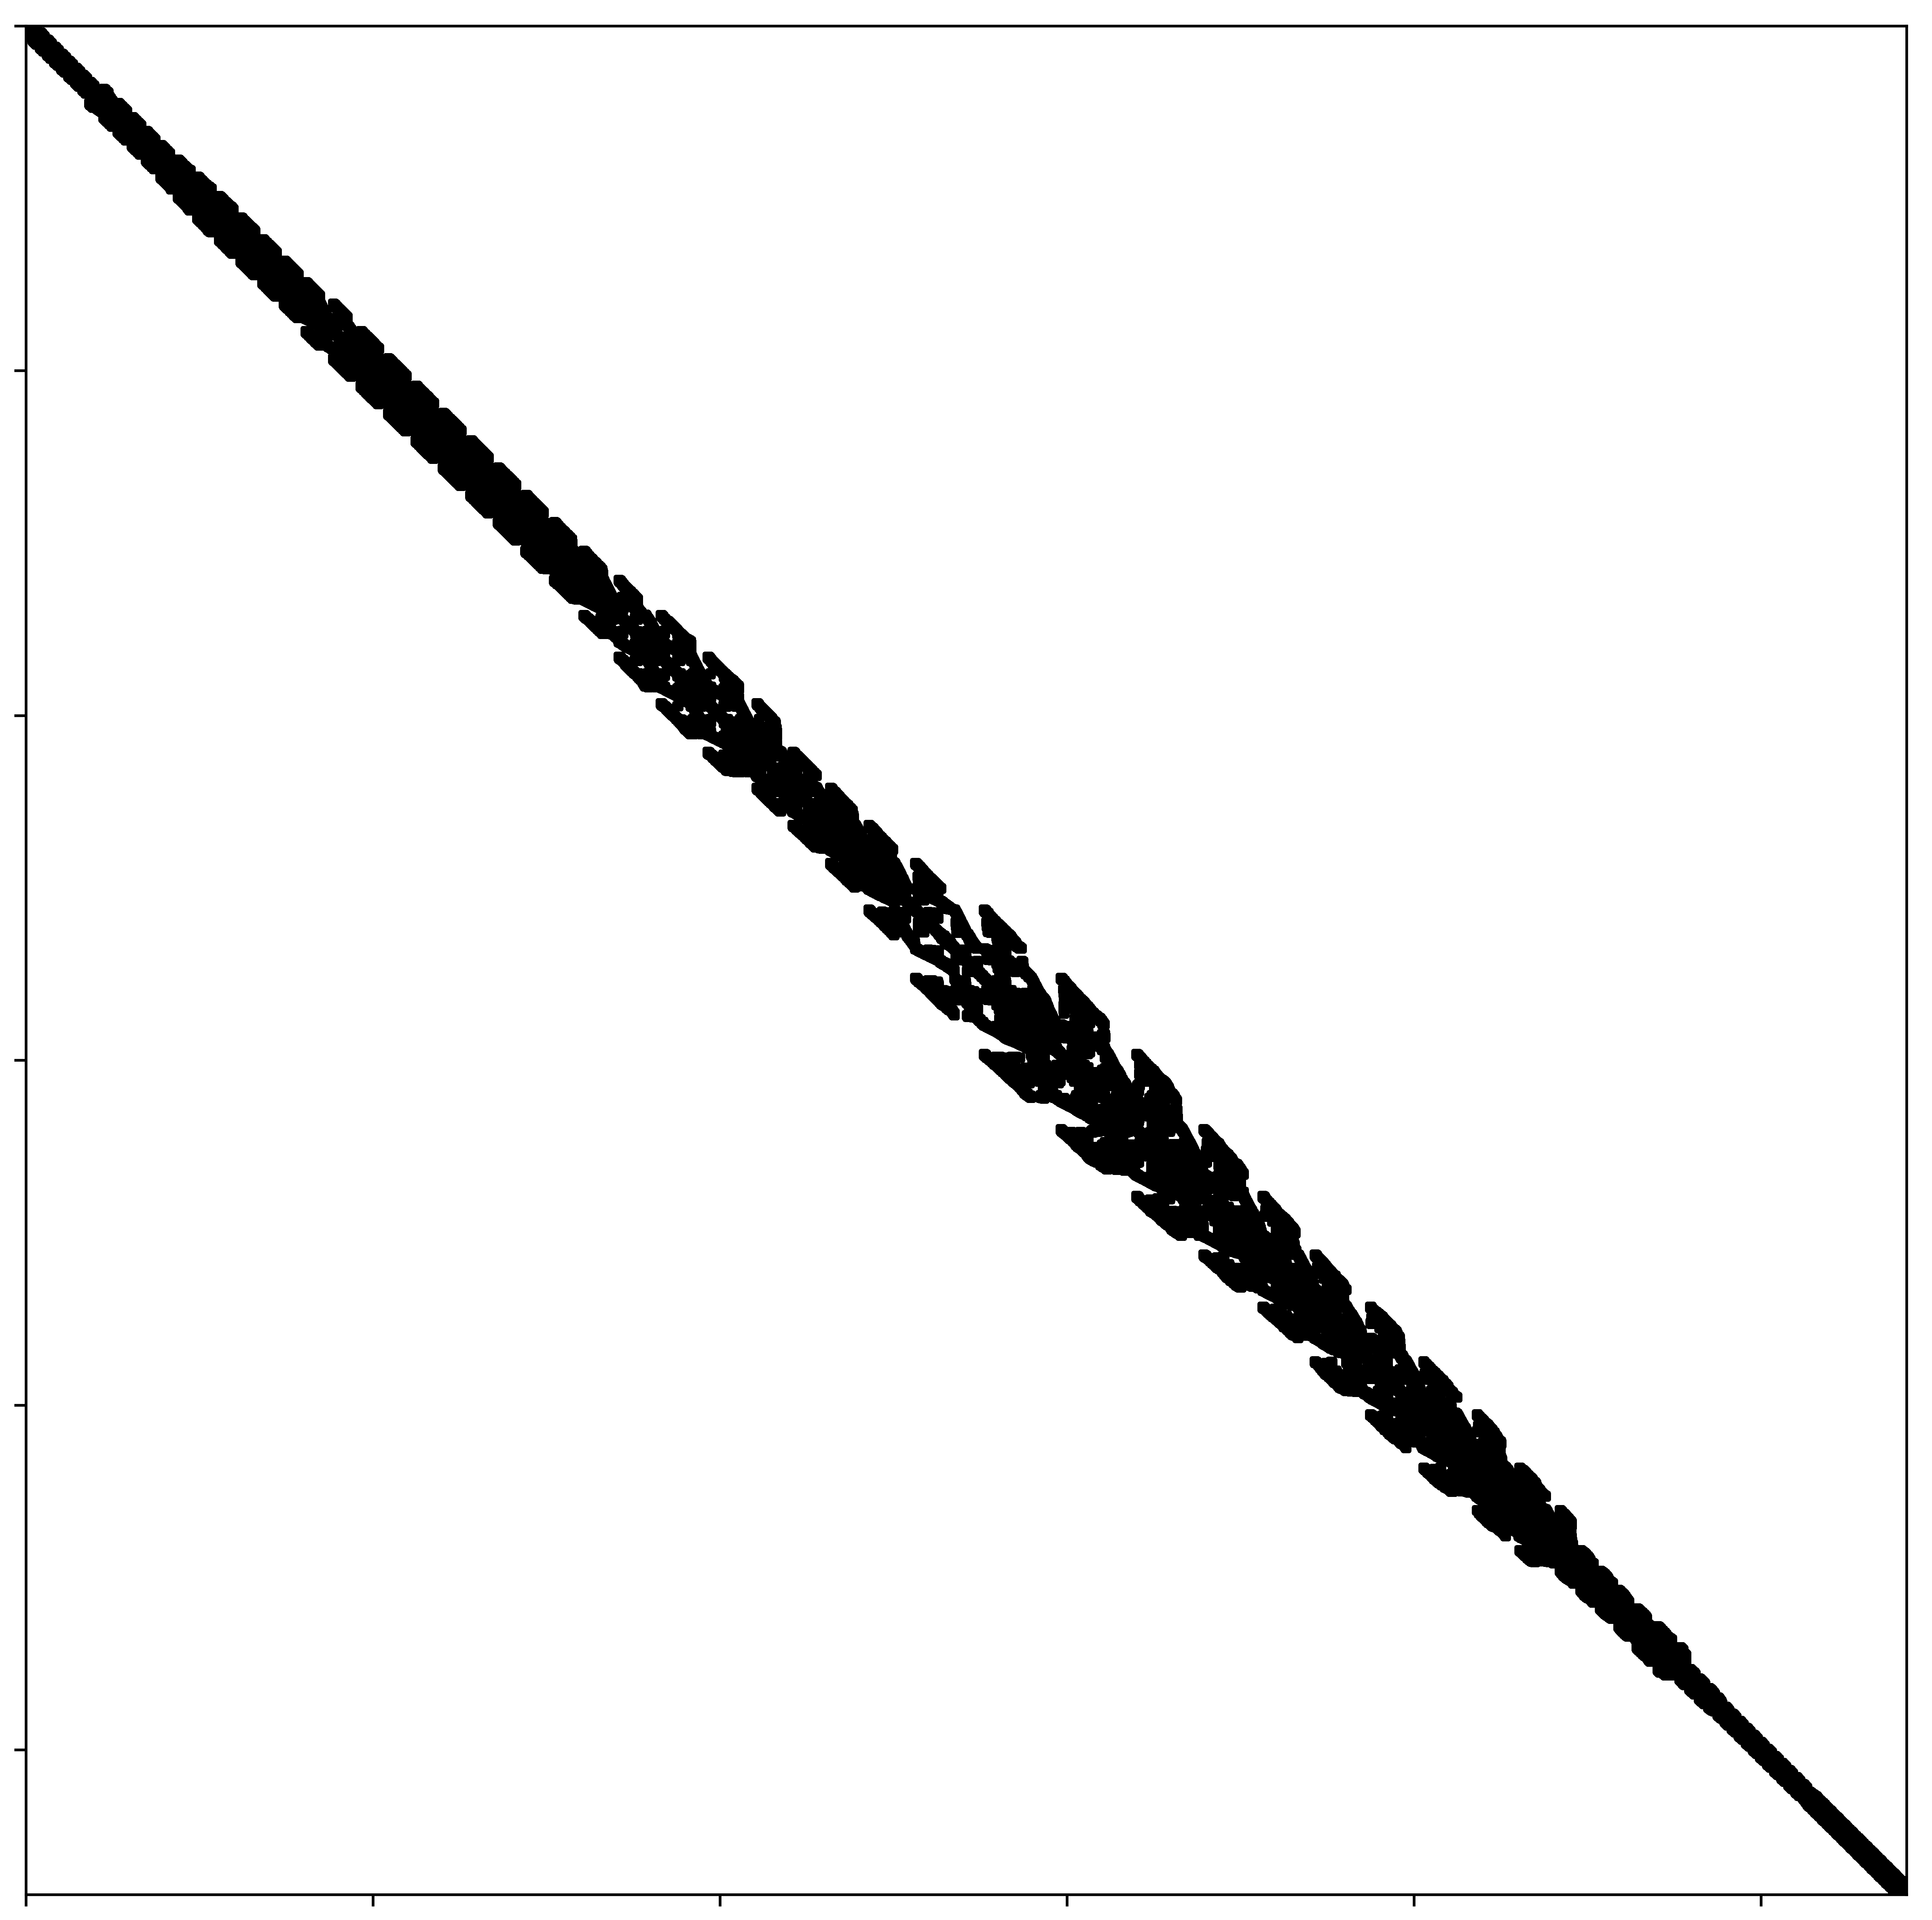
\includegraphics[width=0.32\textwidth]{figures/sparsity-patterns/x104.png}} \\
	\end{tabular}
	\caption{Sparsity patterns of SuiteSparse matrix set}
	\label{fig:sparsity-pattern-suitesparse}
\end{figure}